\documentclass{article}
\usepackage{amsmath}
\usepackage{empheq}
\usepackage{graphicx}
\usepackage[margin=2.54cm]{geometry}
\usepackage{amssymb}
\usepackage{tikz}
\usetikzlibrary{arrows.meta}
\graphicspath{ {../../img/} }
\setlength{\jot}{8pt}

\title{Tarea 1}
\author{Daniel Ise}
\date{Abril 2024}

\begin{document}
\begin{titlepage}
    \begin{center}
        \vspace*{.5cm}
        \includegraphics[scale=.5]{img/udemm-logo.png}\\
        \vspace{.2cm}
        \Large
        \textbf{Facultad de Ingeniería}\\
        \textbf{Ingeniería en Sistemas}\\
        \vspace{2cm}

        \Huge
        Análisis de Sistemas II \\
        Examen Parcial I \\
        Iteración N\(^\circ\) 2 \\
        \vfill

        \raggedright
        \Large
        Docentes:
        \begin{itemize}
            \item[] Mg. Margarita Castronuovo \\
        \end{itemize}
        Alumno:
        \begin{itemize}
            \item[] Daniel Ise
        \end{itemize}
        Legajo:
        \begin{itemize}
            \item[] 28547
        \end{itemize}
        Fecha:
        \begin{itemize}
            \item[] Mayo, 2025
        \end{itemize}
    \end{center}
\end{titlepage}

\section*{Actividad 1}
\begin{enumerate}
	\item[] A) 
	\begin{align*}
		3[ 6x - 5(x-3)] &= 15 - 3(x-5)\\
		3[6x-5x+15)]&=15-3(x-5)\\
		18x-15x+45 &= 30 - 3x\\
		3x + 3x &= 30 - 45\\
		6x &= -15\\
		x &= -\frac{5}{2}
	\end{align*}

	\item[] B)
	\begin{align*}
		\frac{2}{3} \left[ 2(x+1) - \frac{x+1}{2} \right] &= 5 \left( \frac{x}{2} - \frac{2x - 1}{6}\right) \\
		\frac{2}{3} \left[ 2x+2 - \frac{1}{2}x - \frac{1}{2} \right] &= \frac{5}{2}x - \frac{5}{6}(2x-1)  \\
		\frac{4}{3}x + \frac{4}{3} - \frac{1}{3}x - \frac{1}{3} &= \frac{5}{2}x - \frac{5}{3}x + \frac{5}{6}\\
		x+1 &= \frac{15-10}{6}x + \frac{5}{6}\\
		\frac{1}{6}x &= - \frac{1}{6}\\
		x&=-1\\
	\end{align*}

	\item[] C)
	\begin{align*}
		\frac{1}{3}x + \frac{14}{5} - x &= \frac{1}{6} - \frac{7}{10}x \\
		- \frac{2}{3}x + \frac{7}{10}x &= \frac{1}{6} - \frac{14}{5}\\
		\frac{-20+21}{30}x &= \frac{5-84}{30}\\
		\frac{1}{30}x &= - \frac{79}{30}\\
		x &= -79
	\end{align*}

	\item[] D)
	\begin{align*}
		\frac{\sqrt{3x+10}+1}{2-\sqrt{x-3}} &= 2^{0} + 1\\
		\sqrt{3x+10}+1 &= 2 \left( 2-\sqrt{x-3} \right)\\
		\left( \sqrt{3x+10} \right)^{2} &= \left( 3-\sqrt{4x-12} \right)^{2}\\
		3x+10 &= 9 - 6\sqrt{4x-12} + 4x - 12\\
		-x + 13 &= - \sqrt{144x - 432}\\
		(x + 13)^{2} &= (\sqrt{144x - 432})^{2}\\
		x^2 - 26x + 169 &= 144x - 432\\
		x^2 - 170x + 601 &= 0\\
		\frac{170 \pm \sqrt{170^2 - 4 \cdot 1 \cdot 601}}{2} &\Rightarrow x_{1}\approx 166.39 | x_{2} \approx 3.612\\
	\end{align*}

	Sin embargo, controlando con ambos valores no habría igualdad, por lo que las soluciones de $D \not\in \mathbb{R}$

	\item[] E)
	\begin{align*}
		\sqrt{x-2} &= 4\\
		x-2 &= 16\\
		x &= 18
	\end{align*}

	\item[] F)
	\begin{align*}
		x - \frac{3}{2} + \left( 1 - \frac{3}{4} \right)^{\frac{1}{2}} &= (-2)^{-1} - 6(3-x)\\
		x - \frac{3}{2} + \frac{1}{2} &= - \frac{1}{2} - (18 - 6x)\\
		x-1 &= - \frac{1}{2} - 18 + 6x\\
		6x-x &= 18 + \frac{1}{2} - 1\\
		5x &= \frac{35}{2}\\
		x &= \frac{35}{10}
	\end{align*}

	\item[] G)
	\begin{align*}
		\frac{2-(1-x)}{3} - x &= 1 - \frac{2}{3} x\\
		\frac{2}{3} - \frac{1}{3} + \frac{1}{3}x - x &= 1 - \frac{2}{3}x\\
		\frac{1}{3} - \frac{2}{3}x &\neq 1 - \frac{2}{3}x
	\end{align*}

	No tiene solución porque la igualdad es falsa.

\end{enumerate}

\section*{Actividad 2}
\begin{enumerate}
	\item[] A) 
	\begin{align*}
		(x-1)^{2} - 7 &> (x-2)^{2}\\
		x^2 - 2x +1 - 7 &> x^2 -4x +4\\
		-2x+4x &> 4+7-1\\
		2x &> 10\\
		x &> 5
	\end{align*}

	El conjunto solución $S=\left\{ x / x > 5 \right\}$. 
	En forma de intervalo se puede expresar como $(5;+\infty)$.

	Gráficamente:
	\vspace{1cm}

	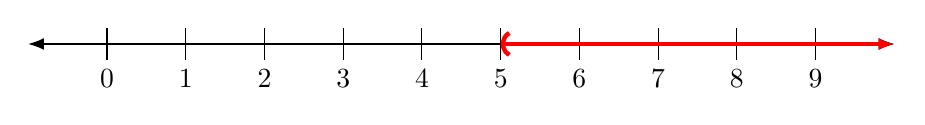
\begin{tikzpicture}
    %\draw[help lines,dashed] (-1,0) grid (10,7); % helper grid OPTIONAL 
    
	\draw[{Latex[length=2mm]}-{Latex[length=2mm]}] (-1,0)-- (10,0); %draw the horizontal axis
    \foreach \x in {0,...,9} {
        \draw (\x,0.2) -- (\x,-0.2) node[below] {\x}; % draw the ticks
    }
		\draw [{Parenthesis[red]}-{Latex[length=2mm]}, ultra thick,color=red] (5, 0) -- (10, 0);
    \end{tikzpicture}

\end{enumerate}

\end{document}
